\documentclass[11pt, a4paper]{article}
\usepackage{rminterim}
\begin{document}

% Your project title etc goes here
\title{\textbf{\textsc{\Huge Writing technical documents}}\\ 
        {\Large Interim Report for Research Project Module 5E1}
      }
\author{Anil Kokaram \\ 
        Trinity College Dublin \\
        {\tt anil.kokaram@tcd.ie}
        }
%\address{Probably not needed}

\date{October 2018}

\maketitle

% This just shows you how to make a manually reformatted section within a page .. which functions like an independent page.
% Its really useful if you want to highlight something and you can even box it up with \fbox 
% You will need this declaration at the start of your report.
\begin{center}
\fbox{\begin{minipage}[t]{0.8\linewidth}
\textit{
This report is submitted in part fulfilment for the assessment required in 5E1 Research Project.  I have read and I understand the plagiarism provisions in the General Regulations of the University Calendar for the current year. These are found in Parts II and III at \myhref{http://www.tcd.ie/calendar}{ http://www.tcd.ie/calendar}.}
\end{minipage}}
\end{center}

% You might not want an abstract so this is up to you
% Just comment it out and use it.
%\begin{abstract}
%An abstract might go here if necessary. An abstract might go here if necessary. An abstract might go here if necessary. An abstract might go here if necessary. An abstract might go here if necessary. An abstract might go here if necessary.
%\end{abstract}

Since 2000, academics at the University have been discussing the need for explicit instruction about scientific writing. Attempts have been made on an ad-hoc basis usually within research groups. This did not address the need at the undergraduate or taught graduate level. Designing modules that satisfy the requirements across all of Engineering and Computer Science resulted in dilution of the message. In this report we present the current state of progress and address pedagogical\footnote{Usually people use this word when they want to hide something about teaching.} concerns with the process. It begins with some background and then gets into the details of Latex. {\bf THE MAIN SECTIONS IN THIS DOCUMENT WERE WRITTEN WITH YOUR INTERIM REPORT IN MIND.}

\section{Introduction}

There is a wealth of online information about scientific writing. It is perhaps better to curate rather than to ignore these sources. Reliable information can be found at the following sites.
 \begin{itemize}
     \item \myhref{https://ieeexplore.ieee.org/stamp/stamp.jsp?tp=&arnumber=4490209}{Effective Communication: Tips on Technical Writing} \cite{malvar_2008}. Written for the IEEE by a famous engineer.
     \item \myhref{https://www.nature.com/scitable/topicpage/effective-writing-13815989/}{Effective Writing} Extremely good information from the journal {\bf Nature}.
     \item \myhref{https://ieeexplore.ieee.org/stamp/stamp.jsp?tp=&arnumber=6955926}{Tips on Scientific Writing and Manuscript Preparation} \cite{linte_2016}. More at the IEEE.
     \item \myhref{https://www.spiedigitallibrary.org/ebooks/PM/How-to-Write-a-Good-Scientific-Paper/eISBN-9781510619142/10.1117/3.2317707}{How to write a good scientific paper}. An SPIE document.
    \item	\myhref{https://www.ncbi.nlm.nih.gov/pmc/articles/PMC3715443/}{Ten Simple Rules for Writing a Literature Review}. This is written for natural sciences but there are some nuggets here for all readers.
    \item \myhref{https://www.springer.com/cda/content/document/cda_downloaddocument/Free+Download+-+Useful+Phrases.pdf?SGWID=0-0-45-1543172-p177775190}{English for writing research papers : Useful Phrases}. A free download from Springer Verlag, one of the most well reputed academic publishers.
 \end{itemize}
 
\subsection{Mathematics}
Ipso facto verum est. Here is an example of some mathematics.
\begin{equation}
    x_1 = \sum_{n=-4}^{N-1} \theta_n + 2\pi x_n - \int_{t=-\infty}^{\infty} \epsilon(t) dt \label{equationofmarking}
\end{equation}
Equation~\ref{equationofmarking} shows how a person can overcome his fear of marking.
\begin{figure}
  \begin{center}
  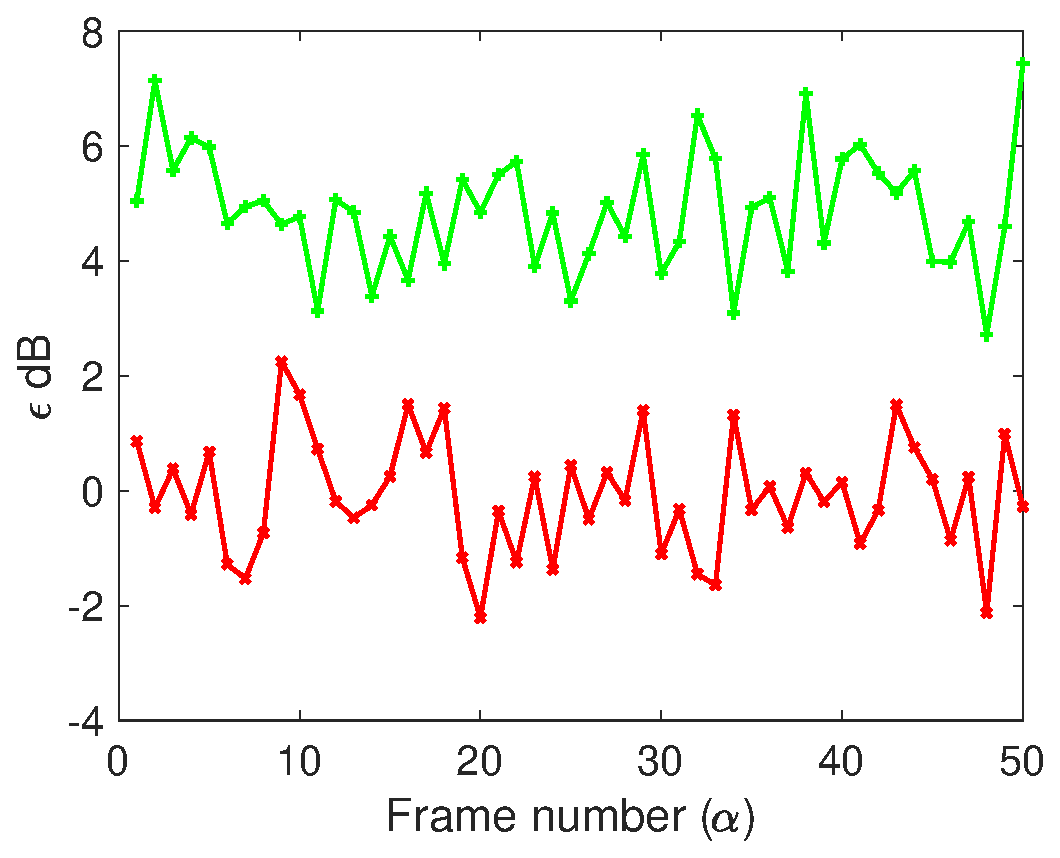
\includegraphics[width=0.7\linewidth]{alineplot.eps}
  \end{center}
  \caption{The distribution of mean squared errors from a difference as in equation~\ref{equationofmarking}. \label{bars}}
  \caprule %\noindent\rule{\linewidth}{0.5pt}
  \end{figure}
\section{Project Objectives}
Ms Ann MacNamara in her course notes \cite{schafer_1996} states that all things are equal. Figure~\ref{bars} illustrates this equality.

\section{Previous Work}
This is the review section. It is here that you build the context from which your work evolves.
Be careful how you search for previous work. Start with Google yes, but recall that there are trusted sources e.g. IEEE, Elsevier, ACM, Springer. Beware of ArXiv. It contains technical reports lodged to maintain authors claims of being first. They are not necessarily peer reviewed. The {\em related links} hyperref in a Google search is quite powerful, but be careful of the \myhref{https://www.youtube.com/watch?v=d3A3-zSOBT4}{Inception} problem.

Do not cite web pages in your bibliography. Use a footnote to reference them if you have to. Citations need to be reproducible over time. So some material from Leicester University in a web site may not be bad but better referenced as a footnote\footnote{\myhref{https://www.le.ac.uk/oerresources/ssds/writingskills/page\_65.htm}{Leicester University Page on Scientific Writing}}. In contrast, a paper on scientific writing by Malvar \cite{malvar_2008} published in the IEEE deserves a citation in the bibliography.


 
 \subsection{Making good plots}
 There is an art to rendering good plots for your document regardless of the document processor being used. Remember to make all lines and text visible at the scale it will be rendered. That often means changing the size of fonts on axes and line thicknesses in plots. Beware of whitespace when rendering images. That causes your plot to occupy less area than you think it should. In Matlab for instance, when rendering an image for inclusion in a document. The following is recommended.
\begin{center}
 \begin{minipage}{\textwidth}
    \begin{verbatim}
      % Render an image in figure 1 (for instance)
      figure(1); 
      image(pic); 
      % Make the picture occupy all the real estate in the figure window
      axis off; 
      set(gca, 'position', [0.01 0.01 0.98 0.98]);
      % Render the picture to an .eps file
      print -depsc mypic.eps  
    \end{verbatim}
 \end{minipage}
\end{center}

% An example of two figures side by side
\begin{figure}
\centering
\begin{minipage}{0.45\textwidth}
\centering 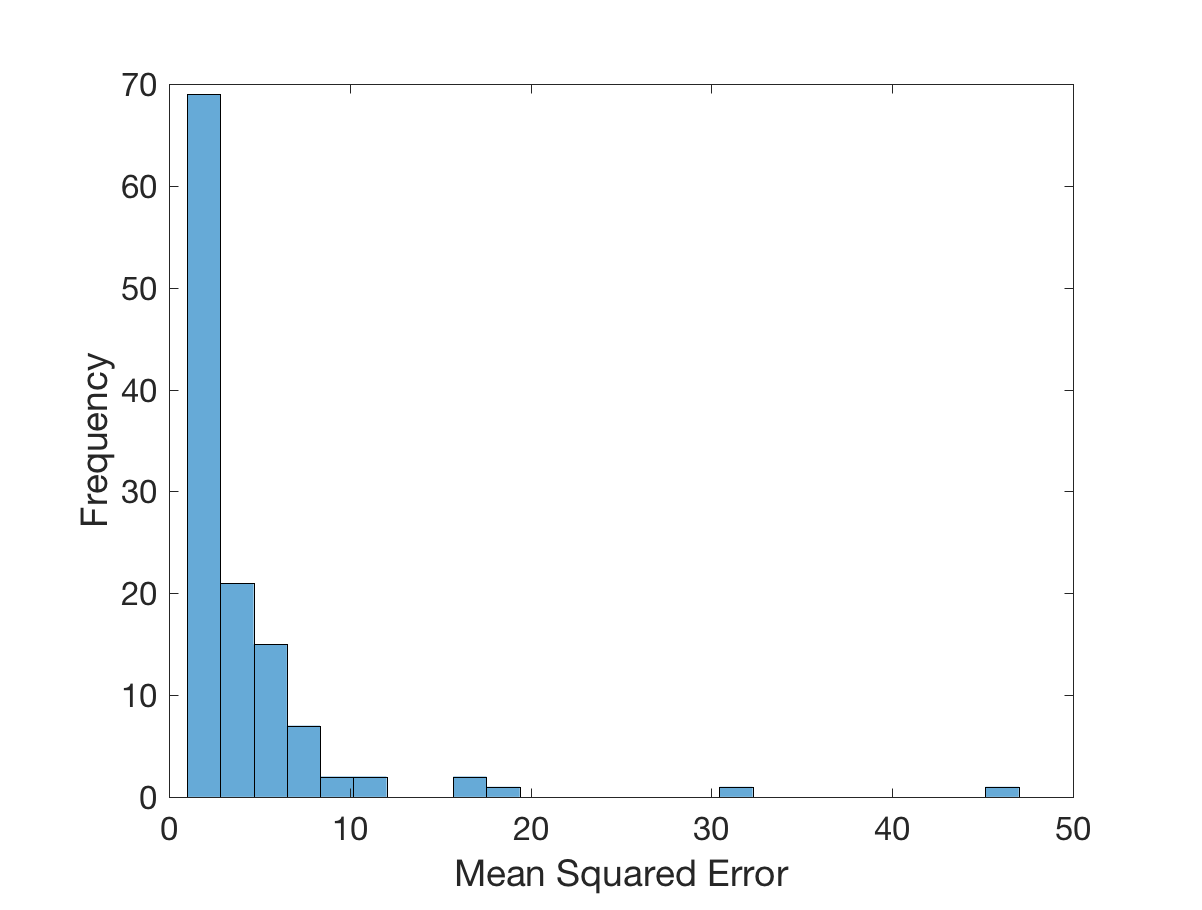
\includegraphics[width=\linewidth,]{bars.eps}
\end{minipage} \hspace*{0.25cm}
\begin{minipage}{0.45\textwidth}
\centering 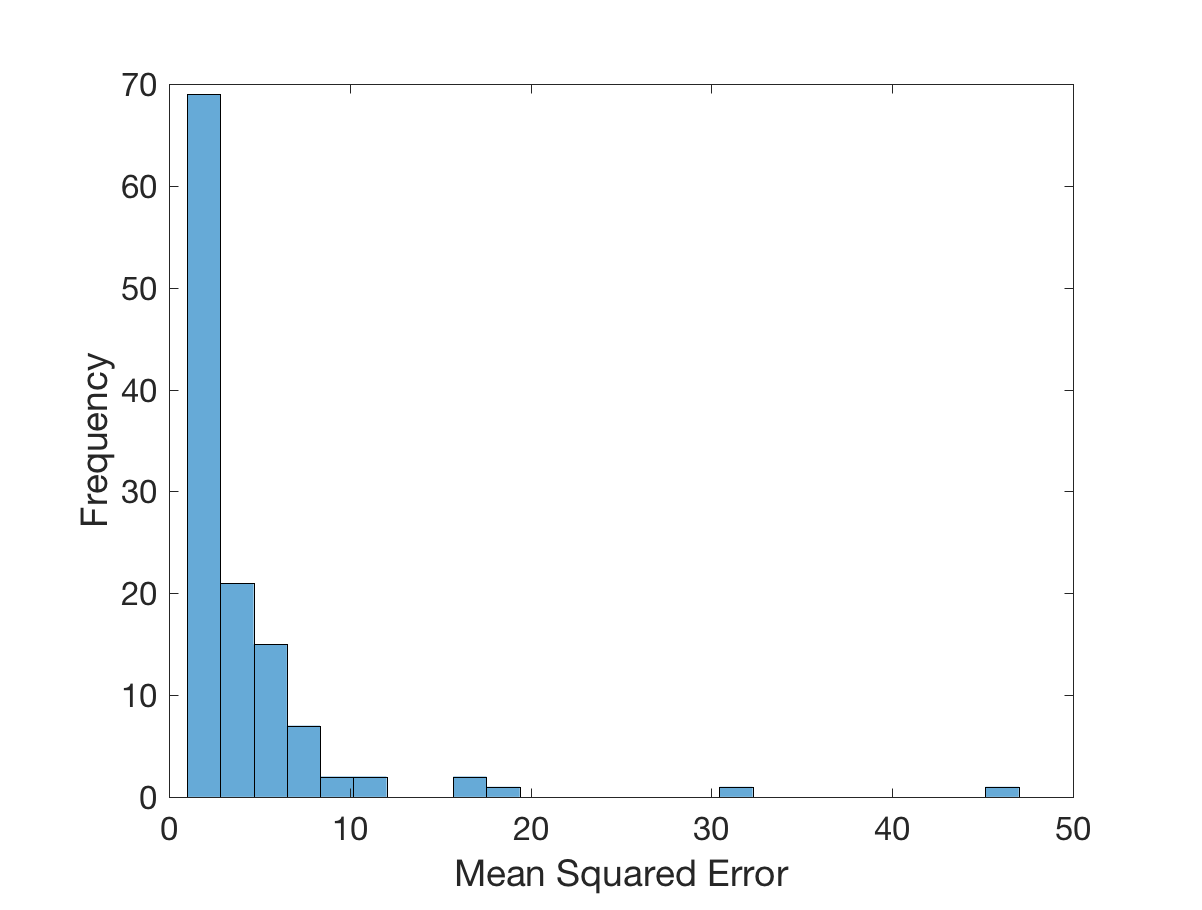
\includegraphics[width=\linewidth,]{bars.eps}
\end{minipage}
\caption{Left : Distribution of temperature measurements in the orbiting satellite. Right : Distribution of humidity in the spacecraft as a difference from target. \label{twofigs}}
\caprule
\end{figure}


Here is an example of some mathematics.
\begin{equation}
    x_1 = \sum_{n=-4}^{N-1} \theta_n + 2\pi x_n - \int_{t=-\infty}^{\infty} \epsilon(t) dt \label{equationofmarking2}
\end{equation}
Equation~\ref{equationofmarking2} shows how a person can overcome his fear of marking.

\section{Ethical Considerations}

\section{Progress to Date}
Several new experiments have been run in Semester I of 2019/20. They involve a cohort of more than 100 students. Results indicate an improvement of 25\% over 50\% of the cohort and 55\% over 25\% of the cohort. 

\section{Self Assessment}

\section{Project Plan}
Methodology follows all the work that went before \cite{dirac,boykov_2001}

\subsection{Expected Results and Challenges}
Provided that the models proposed are accurate we expect to observe a low error against our targets. This can be measured by plotting X and Y.

% Here are my references
\bibliographystyle{acm}
\bibliography{myrefs}

\end{document}
